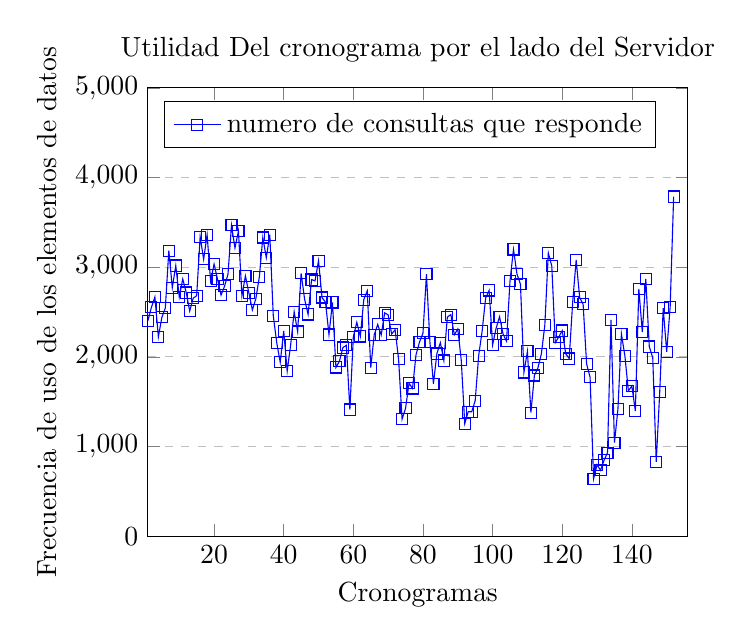
\begin{tikzpicture}
\begin{axis}[
    title={Utilidad Del cronograma por el lado del Servidor},
    xlabel={Cronogramas},
    ylabel={Frecuencia de uso de los elementos de datos},
    xmin=1, xmax=156,
    ymin=0, ymax=5000,
    xtick={},
    ytick={},
    legend pos=north west,
    ymajorgrids=true,
    grid style=dashed,
]

\addplot[
    color=blue,
    mark=square,
    ]
    coordinates {
%UTILIDAD TOTAL
(1,2404)
(2,2553)
(3,2667)
(4,2224)
(5,2440)
(6,2545)
(7,3185)
(8,2771)
(9,3018)
(10,2668)
(11,2868)
(12,2717)
(13,2511)
(14,2655)
(15,2681)
(16,3340)
(17,3088)
(18,3362)
(19,2844)
(20,3035)
(21,2864)
(22,2689)
(23,2787)
(24,2924)
(25,3467)
(26,3215)
(27,3403)
(28,2680)
(29,2903)
(30,2712)
(31,2523)
(32,2649)
(33,2891)
(34,3331)
(35,3106)
(36,3363)
(37,2460)
(38,2157)
(39,1939)
(40,2288)
(41,1841)
(42,2135)
(43,2503)
(44,2282)
(45,2931)
(46,2644)
(47,2473)
(48,2862)
(49,2848)
(50,3072)
(51,2662)
(52,2610)
(53,2249)
(54,2607)
(55,1882)
(56,1952)
(57,2104)
(58,2129)
(59,1412)
(60,2226)
(61,2385)
(62,2228)
(63,2638)
(64,2736)
(65,1880)
(66,2246)
(67,2362)
(68,2243)
(69,2490)
(70,2468)
(71,2255)
(72,2302)
(73,1972)
(74,1306)
(75,1426)
(76,1706)
(77,1648)
(78,2023)
(79,2165)
(80,2264)
(81,2921)
(82,2163)
(83,1700)
(84,2037)
(85,2158)
(86,1959)
(87,2444)
(88,2471)
(89,2246)
(90,2311)
(91,1961)
(92,1255)
(93,1389)
(94,1387)
(95,1512)
(96,2014)
(97,2289)
(98,2657)
(99,2741)
(100,2134)
(101,2318)
(102,2448)
(103,2255)
(104,2174)
(105,2847)
(106,3198)
(107,2924)
(108,2811)
(109,1826)
(110,2061)
(111,1378)
(112,1792)
(113,1875)
(114,2032)
(115,2352)
(116,3159)
(117,3013)
(118,2158)
(119,2222)
(120,2293)
(121,2035)
(122,1981)
(123,2611)
(124,3080)
(125,2664)
(126,2586)
(127,1921)
(128,1772)
(129,640)
(130,797)
(131,735)
(132,846)
(133,931)
(134,2412)
(135,1043)
(136,1418)
(137,2256)
(138,2009)
(139,1620)
(140,1675)
(141,1395)
(142,2758)
(143,2277)
(144,2868)
(145,2115)
(146,1990)
(147,828)
(148,1608)
(149,2543)
(150,2057)
(151,2558)
(152,3788)
    };
    \legend{numero de consultas que responde}

\end{axis}
\end{tikzpicture}

